\documentclass[a4paper]{article}
\usepackage{a4wide}
\usepackage{amsmath}
\usepackage{graphicx}
\usepackage{indentfirst}
% \usepackage[spanish]{babel}
\usepackage{amsfonts}
\usepackage{hyperref}
\usepackage{tikz,pgfplots}
\usepackage[mathcal]{eucal}

\usepackage[usenames,dvipsnames]{pstricks}
\usepackage{epsfig}
\usepackage{pst-grad} % For gradients
\usepackage{pst-plot} % For axes
\usepackage[space]{grffile} % For spaces in paths
\usepackage{etoolbox} % For spaces in paths
\makeatletter % For spaces in paths
\patchcmd\Gread@eps{\@inputcheck#1 }{\@inputcheck"#1"\relax}{}{}
\makeatother
\usepackage[abs]{overpic}
\setlength\unitlength{1mm}

\newcommand{\Z}{\mathbb{Z}}
\newcommand{\angstrom}{\textup{\AA}}

\renewcommand\contentsname{\'Indice}
\renewcommand\figurename{Figura}

\begin{document}
\title{Recubrimientos antirreflectivos}
\author{P. Cobelli}
\date{Fecha de \'ultima actualizaci\'on: 22 de Noviembre de 2015}
\maketitle

\noindent\makebox[\linewidth]{\rule{\textwidth}{0.4pt}}
\tableofcontents
\vspace{0.4cm}
\noindent\makebox[\linewidth]{\rule{\textwidth}{0.4pt}}

\section{Antes de comenzar}

Asumamos por un momento que las lentes de las que est\'an compuestos nuestros
anteojos forman, con el aire, dos interfaces que pueden considerarse planas y
paralelas entre s\'\i .

Una de estas dos interfaces es la que denominaremos {\it frontal} o {\it 
anterior}, 
corresponde a la interfaz aire-vidrio por la que los rayos de luz que se 
dirigen hacia nuestros ojos ingresan en el material del que est\'an hechas 
las lentes. La segunda interfaz, vidrio-aire,  es la llamada {\it posterior}, 
y corresponde a aquella que es m\'as cercana a nuestros ojos. 

Bajo la hip\'otesis de que estas dos interfaces son planas y paralelas, 
un lector desprevenido podr\'\i a pensar que los rayos por ellas reflejados (o 
transmitidos) ser\'\i an capaces de dar lugar a interferencia. Sin embargo 
sabemos que esto no es posible dado que el espesor de dicha l\'amina supera
ampliamente la longitud de coherencia necesaria para observar interferencia.

\section{El principio de funcionamiento}

La idea detr\'as de los recubrimientos antireflectivos es que es posible crear
una l\'amina {\it delgada} de caras paralelas por delante de la superficie
frontal de nuestras lentes, de forma tal de que para cada rayo incidente 
haya dos rayos reflejados susceptibles de interferir entre s\'\i . 

En particular, si somos capaces de hacer que estos dos rayos reflejados 
se encuentren en contrafase, su interferencia podr\'\i a dar lugar a una
cancelaci\'on parcial o total\footnote{Volveremos sobre este punto en la
Secci\'on 3.} de la intensidad luminosa reflejada. 

Consideremos entonces el sistema f\'\i sico que se muestra en la Fig.~\ref{fa}.
En el mismo se representa, en forma esquem\'atica, la pel\'\i cula delgada
de recubrimiento dispuesta delante de la lente. Asumiremos que el espesor
de la capa de recubrimiento es $d$ y su \'\i ndice de refracci\'on viene 
dado por $n_r$. Asimismo, consideraremos que el \'\i ndice de refracci\'on de
la lente del anteojo es $n_l$, y que el material del que est\'an compuestas
es el m\'as denso \'opticamente, es decir: $1 < n_r < n_l$. 

Sobre este arreglo, vamos a considerar la incidencia {\it normal} 
(adecuada para las situaciones en las que utilizamos nuestros anteojos) de 
luz monocrom\'atica de longitud de onda $\lambda_0$. 

\begin{figure}
    \centering
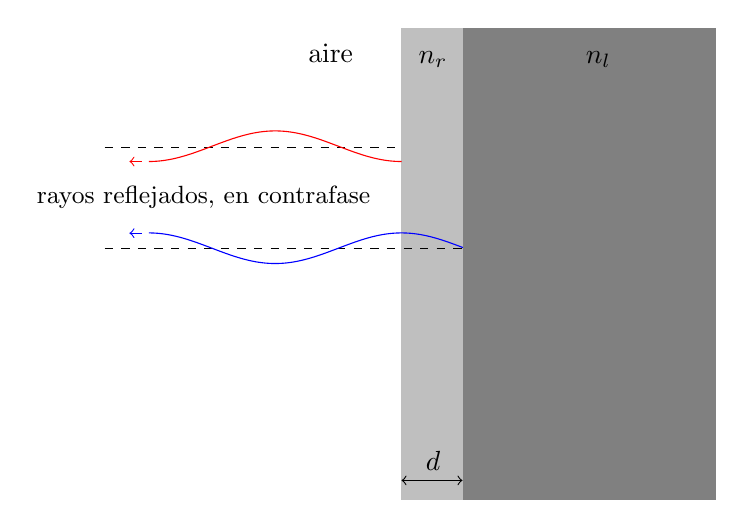
\begin{tikzpicture}
  % lente
  \fill [gray] (1,-3) rectangle (4,3);
  % recubrimiento 
  \fill [lightgray] (0,-3) rectangle (1,3); 
  \draw[<->] (0,-2.75) -- (0.775, -2.75);   
  % ondas
  % ejes cero de las ondas
  \draw[dashed,black] (-1.2*pi,1.475) -- (0,1.475);
  \draw[dashed,black] (-1.2*pi,0.2) -- (1,0.2);
  \begin{axis}[
     hide axis,
     clip=false,
     xmin=0,xmax=2*pi,
     axis lines=none,
     width=8cm,height=3cm
     ]
      \addplot[domain=-3*pi/4:0,samples=1000,red]{-0.15*cos(deg(2*x))+1};
      \addplot[domain=-3*pi/4:1,samples=1000,blue]{0.15*cos(deg(2*x))};
      \addplot[domain=-pi:-3*pi/4,samples=250,blue]{0.15*cos(deg(2*x))};
      \addplot[domain=-pi:-3*pi/4,samples=1000,red]{-0.15*cos(deg(2*x))+1};
  \end{axis}
  % flechas
  \draw[<-,red] (-1.1*pi,1.3)--(-1.05*pi,1.3);
  \draw[<-,blue] (-1.1*pi,0.39)--(-1.05*pi,0.39);
  \fill [gray] (0.775,-3) rectangle (4,3);
  % textos
  \node[] at (-0.8*pi,0.85) {{\small rayos reflejados, en contrafase}};
  \node[] at (0.4,-2.5) {$d$};
  \node[] at (-0.9,2.67) {aire};
  \node[] at (0.4,2.6) {$n_r$};
  \node[] at (2.5, 2.6) {$n_l$};
\end{tikzpicture}%
\hspace{1cm}
\includegraphics[scale=0.7]{ojo.jpg}
\vspace{0.5cm}
\caption{Esquema para el an\'alisis del funcionamiento de los recubrimientos
antireflectivos. El esquema muestra un modelo idealizado de recubrimiento
de \'\i ndice $n_r$ en la forma de una pel\'\i cula delgada de espesor
$d$, dispuesto delante de
la lente de \'\i ndice de refracc\'on $n_l$. Los rayos de luz llegan a 
nuestros ojos provenientes de la izquierda. Se observan tambi\'en dos 
rayos reflejados, uno por la interfaz aire-recubrimiento (en rojo) y otro
por la interfaz recubrimiento-lente (en azul). Cuando ambos emergen en
contrafase (como se muestra en la figura) se produce interferencia 
destructiva (parcial o total, seg\'un el caso).}
\label{fa}
\end{figure}

Buscamos entonces una condici\'on que nos permita asegurar que la onda
reflejada por la interfaz aire-recubrimiento (en rojo en la Fig.~\ref{fa})
interfiera destructivamente con aquella reflejada por la interfaz 
recubrimiento-lente (en azul en la misma figura). Estas dos ondas son las
reflejadas en las caras anterior y posterior de una l\'amina delgada de 
caras paralelas de material con \'\i ndice $n_r$ entre aire y el vidrio del
que est\'an hechas las lentes. 

Calculemos entonces la diferencia de fase entre ambos rayos. Por un lado, 
la diferencia de camino geom\'etrico entre ambos se debe exclusivamente a
que la onda transmitida (en azul en el esquema) atraviesa dos veces el espesor
de la l\'amina, luego el camino geom\'etrico extra que el rayo {\it azul}
recorre respecto del {\it rojo} es $2 d$. Dado que el medio en el que tiene
lugar este camino tiene \'\i ndice $n_r$, la diferencia de camino \'optico
entre los rayos {\it rojo} y {\it azul} es $2 n_r d$. Finalmente, la diferencia
de fase entre ambos resulta
\begin{equation*}
    \delta' = k \cdot 2 n_r d = \frac{4 \pi}{\lambda_0} n_r d.
\end{equation*}
Esta diferencia de fase $\delta'$ est\'a asociada {\it exclusivamente} a las
diferencias de camino entre ambos rayos interfirientes. Es decir que para 
determinar la diferencia de fase total $\delta$ es necesario considerar los
posibles saltos de fase en las interfaces. 

En la interfaz aire-recubrimiento, la luz pasa de un medio de \'\i ndice dado 
a otro de \'\i ndice mayor, por lo que el rayo reflejado (en rojo)
experimenta un salto de fase de $\pi$ radianes. Lo mismo sucede en la interfaz
recubrimiento-lente,
dado que estamos trabajando bajo la hip\'otesis de que $n_r < n_l$. Por lo 
tanto, la diferencia de fase proveniente de saltos de fase por 
reflexi\'on es de $2 \pi$ radianes. 

Luego la diferencia de fase entre ambos rayos en incidencia normal viene 
dada por
\begin{equation}
    \delta = \frac{4\pi}{\lambda_0} n_r d + 2\pi.
\end{equation}

Si ambos rayos presentan la misma intensidad luminosa, la condici\'on de
interferencia destructiva resulta 
\begin{equation*}
    \cos^2 \delta/2 = 0 \quad \quad \Rightarrow \quad \quad \delta = (2m+1)\pi,
    \quad \quad m \in \Z_0.
\end{equation*}
A partir de esta condici\'on resulta sencillo encontrar los espesores de capa
de recubrimiento $d_m$ posibles en t\'erminos de los par\'ametros relevantes 
del sistema:
\begin{equation}
    d_m  = \frac{2m+1}{4} \: \frac{\lambda_0}{n_r}.
\end{equation}
Esta condici\'on nos asegura que no habr\'a luz reflejada a partir de la capa 
de recubrimiento depositada sobre nuestras lentes. Los espesores posibles
resultan entonces:
\begin{equation*}
    d_m = \{ 1/4 (\lambda_0/n_r),  3/4 (\lambda_0/n_r), 5/4 (\lambda_0/n_r), 
    \ldots \}
\end{equation*}
No obstante, sabemos que si el espesor resulta muy grande las ondas
interfirientes podr\'\i an perder coherencia y nuestro sistema dejar\'\i a de
funcionar como un filtro antirreflejos. Asimismo, un recubrimiento de mayor
$d$ implica anteojos con vidrios m\'as gruesos y m\'as pesados. Por ende, 
resulta usual considerar el m\'\i nimo espesor de recubrimiento capaz de
asegurar la propiedad de ser antirreflectivo. El m\'\i nimo espesor
posible que cumple con esta condici\'on, simbolizado por $d_\text{min}$,
viene dado por la
expresi\'on:
\begin{equation}
    d_\text{min} = \frac{\lambda_0}{4 \: n_r}.
\end{equation}

\section{C\'omo elegir el material que compone el recubrimiento}

Notemos que, hasta ahora, venimos considerando que la intensidad de ambos
rayos reflejados es la misma. Sin embargo, vimos en las clases te\'oricas
que este no es el caso. Esto se debe a que, cuando un rayo de intensidad
$I_0$ incide {\it normalmente} sobre una interfaz entre dos medios de \'\i ndices
$n_1$ y $n_2$, las intensidades de los haces reflejado y transmitido  vienen
dadas por
\begin{equation}
    I_\text{reflej} = I_0 \: \mathcal{R}_{12} = I_0 \: \left( \frac{n_2-n_1}{n_2 + n_1} \right)^2, \\
\end{equation}
y
\begin{equation}
    I_\text{transm} = I_0 \: \mathcal{T}_{12} = I_0 \: (1-\mathcal{R}_{12}),
\end{equation}\\
siendo $\mathcal{R}_{12}$ la reflectividad de la interfaz 1-2, y
$\mathcal{T}_{12}$ la transmitividad de esa misma interfaz. Observemos que 
$\mathcal{R}_{12} + \mathcal{T}_{12} = 1$, de forma tal de que la intensidad 
asociada al rayo luminoso original se conserva al dividirse en reflejado y transmitido. 
Las \'ultimas expresiones nos muestran que dependiendo del valor
de los \'\i ndices las intensidades
reflejada y transmitida ser\'an, en general, distintas entre s\'\i . 

Por esta raz\'on, el espesor m\'\i nimo que calculamos en la secci\'on anterior
s\'olo asegura una interferencia destructiva {\it parcial} de la luz reflejada,
dado que ambos rayos no tienen la misma intensidad al emerger del recubrimiento.

Para poder obtener una cancelaci\'on total resulta necesario entonces elegir
correctamente el material que compondr\'a el recubrimiento. Veamos c\'omo se
calcula exactamente el \'\i ndice de refracci\'on de ese material de forma tal
de asegurar interferencia destructiva completa de las ondas reflejadas.

\begin{figure}
    \centering
    % \usepackage[usenames,dvipsnames]{pstricks}
% \usepackage{epsfig}
% \usepackage{pst-grad} % For gradients
% \usepackage{pst-plot} % For axes
% \usepackage[space]{grffile} % For spaces in paths
% \usepackage{etoolbox} % For spaces in paths
% \makeatletter % For spaces in paths
% \patchcmd\Gread@eps{\@inputcheck#1 }{\@inputcheck"#1"\relax}{}{}
% \makeatother
% % User Packages:
% 
% 
\psscalebox{1.0 1.0} % Change this value to rescale the drawing.
{
\begin{pspicture}(0,-1.8828238)(6.24,1.8828238)
\definecolor{colour0}{rgb}{0.8,0.8,0.8}
\definecolor{colour1}{rgb}{0.6,0.6,0.6}
\psframe[linecolor=colour0, linewidth=0.04, fillstyle=solid,fillcolor=colour0, dimen=outer](5.792308,0.5823445)(0.2723077,-0.8776555)
\psframe[linecolor=colour1, linewidth=0.04, fillstyle=solid,fillcolor=colour1, dimen=outer](5.792308,-1.6)(0.2723077,-0.8776555)
\psline[linecolor=black, linewidth=0.04, arrowsize=0.05291667cm 2.0,arrowlength=1.4,arrowinset=0.0]{->}(0.35384616,1.5777291)(1.7384615,0.60849833)
\psline[linecolor=green, linewidth=0.04, arrowsize=0.05291667cm 2.0,arrowlength=1.4,arrowinset=0.0]{->}(1.7538462,0.5623445)(2.3076923,-0.8530401)
% \psline[linecolor=black, linewidth=0.04, arrowsize=0.05291667cm 2.0,arrowlength=1.4,arrowinset=0.0]{->}(2.3076923,-0.8684247)(3.6923077,-1.8376555)
\psline[linecolor=red, linewidth=0.04, arrowsize=0.05291667cm 2.0,arrowlength=1.4,arrowinset=0.0]{<-}(3.1384616,1.5777291)(1.7538462,0.60849833)
\psline[linecolor=orange, linewidth=0.04, arrowsize=0.05291667cm 2.0,arrowlength=1.4,arrowinset=0.0]{<-}(2.876923,0.5777291)(2.323077,-0.8376555)
% \psline[linecolor=black, linewidth=0.04, arrowsize=0.05291667cm 2.0,arrowlength=1.4,arrowinset=0.0]{->}(2.9076922,0.5777291)(3.4615386,-0.8376555)
% \psline[linecolor=black, linewidth=0.04, arrowsize=0.05291667cm 2.0,arrowlength=1.4,arrowinset=0.0]{<-}(4.0307693,0.5931137)(3.476923,-0.8222709)
\psline[linecolor=blue, linewidth=0.04, arrowsize=0.05291667cm 2.0,arrowlength=1.4,arrowinset=0.0]{<-}(4.292308,1.5777291)(2.9076922,0.60849833)
% \psline[linecolor=black, linewidth=0.04, arrowsize=0.05291667cm 2.0,arrowlength=1.4,arrowinset=0.0]{<-}(5.4,1.5623446)(4.0153847,0.5931137)
\rput[red](2.7538462,1.6546522){$I_\text{rayo1}$}
\rput[blue](4.123077,1.6854215){$I_\text{rayo2}$}
\rput[bl](5.0,0.9469599){}
\rput[bl](0.0,1.6854215){$I_0$}
\rput[bl](4.7,0.8){$\text{aire}$}
\rput[bl](4.7,-0.2){$n_r$}
\rput[bl](4.7,-1.4){$n_l$}
\rput[orange](2.95,-0.2){$I_{s'}$}
\rput[green](1.75, -0.2){$I_{s}$}
\end{pspicture}
}


    \caption{Esquema de rayos reflejados en las interfaces aire-recubrimiento
    y recubrimiento-lente. En este diagrama, el conjunto recubrimiento-lente
    ha sido rotado a la derecha respecto de la Fig.~\ref{fa}. 
    Las magnitudes $I_0$, $I_\text{rayo1}$, 
$I_\text{rayo2}$, $I_{s}$ e $I_{s'}$ corresponden a las intensidades
    de cada uno de los rayos intervinientes.
    No se muestra el rayo transmitido a la lente producto de la 
refracci\'on del rayo identificado con color verde. }
\label{fig:r2}
\end{figure}

Para esto, vamos a ayudarnos con el diagrama de la Figura~\ref{fig:r2}. 
A pesar de que en el mismo se muestra una incidencia obl\'\i cua de rayos,
nosotros emplearemos el diagrama pens\'andolo para el caso de incidencia
normal, y utilizaremos el trazado en incidencia obl\'\i cua s\'olo para 
poder visualizar f\'acilmente los diferentes rayos de inter\'es, que 
ser\'\i a dif\'\i cil distinguir si hici\'esemos el diagrama en 
incidencia normal. Hecha esta salvedad, la Fig.~\ref{fig:r2} muestra 
un rayo incidente sobre la interfaz aire-recubrimiento
caracterizado por una intensidad $I_0$ (en negro). Ese rayo se 
dividir\'a en uno reflejado hacia el aire (en rojo) 
y otro transmitido hacia el interior de la pel\'\i cula de recubrimiento
(en verde).  
De acuerdo a las definiciones anteriores, el reflejado tendr\'a una intensidad
dada por:
\begin{equation}
    I_\text{rayo1} = I_0 \mathcal{R}_{ar},
\end{equation}
donde $\mathcal{R}_{ar}$ representa la reflectividad de la interfaz 
aire-recubrimiento, y viene dada por
\begin{equation}
    \mathcal{R}_{ar} = \left( \frac{n_r-n_a}{n_r + n_a} \right)^2 =
    \left( \frac{n_r-1}{n_r + 1} \right)^2. 
\end{equation}
El rayo transmitido (en verde) tendr\'a entonces una intensidad
\begin{equation}
    I_s = I_0 \mathcal{T}_{ar} = I_0 \left(1 - \mathcal{R}_{ar}\right).
\end{equation}
A continuaci\'on este \'ultimo rayo se reflejar\'a en la interfaz
recubrimiento-lente, dando lugar a un rayo reflejado que se propaga
en el recubrimiento hacia su interfaz con el aire (rayo naranja en 
la figura). La intensidad de este rayo ser\'a entonces
\begin{equation}
    I_{s'} = I_s \mathcal{R}_{rl},
\end{equation}
siendo $\mathcal{R}_{rl}$ la reflectividad de la interfaz 
recubrimiento-lente:
\begin{equation}
    \mathcal{R}_{rl} = \left( \frac{n_l-n_r}{n_l + n_r} \right)^2.
\end{equation}
Finalmente ese rayo se transmitir\'a a trav\'es de la interfaz 
aire-recubrimiento, dando lugar al rayo esquematizado en azul en la
Figura. Ese rayo tendr\'a entonces una intensidad dada por
\begin{equation}
    I_\text{rayo2} = I_{s'} \mathcal{T}_{ar} = I_{s'} \left( 
    1 - \mathcal{R}_{ar}\right).
\end{equation}

En esta forma, las intensidades de los rayos 1 y 2 (rojo y azul en la
figura) que interfieren vienen dadas por
\begin{equation}
    I_\text{rayo1} = I_0 \: \mathcal{R}_{ar},
\end{equation}
y
\begin{align*}
    I_\text{rayo2} &= I_{s'} \mathcal{T}_{ar} = \\
                   &= I_{s'} \: \left(1 - \mathcal{R}_{ar}\right) = \\
                   &= I_s \: \mathcal{R}_{rl} \left(1 - \mathcal{R}_{ar}\right) =  \\
                   &= I_0 \left(1 - \mathcal{R}_{ar}\right) \: \mathcal{R}_{rl} 
\left(1 - \mathcal{R}_{ar}\right),
\end{align*}
es decir que
\begin{equation}
    I_\text{rayo2} = I_0 \: \mathcal{R}_{rl} \: 
    \left( 1 - \mathcal{R}_{ar}\right)^2.
\end{equation}

Luego, para que estos dos rayos que interfieren tengan la misma 
intensidad, deber\'a suceder que
\begin{equation}
    I_\text{rayo1} = I_\text{rayo2},
\end{equation}
o, lo que es equivalente,
\begin{equation*}
    I_0 \: \mathcal{R}_{ar} = I_0 \: \mathcal{R}_{rl} \: \left(
    1 - \mathcal{R}_{ar}        \right)^2,
\end{equation*}
condici\'on que puede reescribirse como
\begin{equation}
    \mathcal{R}_{ar} = \left(1- 2\: \mathcal{R}_{ar} +
    \mathcal{R}_{ar}^2 \right) \: \mathcal{R}_{rl}.
\end{equation}
En esta ecuaci\'on, $\mathcal{R}_{ra}$ depende de $n_r$ (ecuaci\'on
7), y
$\mathcal{R}_{rl}$ depende de $n_r$ y $n_l$ (ecuaci\'on 10). Por tanto,
esta es una ecuaci\'on algebraica de la que en principio es
posible obtener el valor del \'\i ndice de refracci\'on
del recubrimiento, $n_r$, si se conoce $n_l$. 

Ahora bien, seg\'un vimos en clases te\'oricas, el coeficiente de 
reflectividad\footnote{En incidencia normal.} aire-vidrio es en general bajo, del orden de 0.02 para
un vidrio de \'\i ndice de refracci\'on $n = 1.33$. Esto nos permite
entonces despreciar el segundo y tercer t\'ermino dentro de los 
par\'entesis en la \'ultima ecuaci\'on {\it frente al primer sumando} (que
es igual
a 1), con lo cual la condici\'on
aproximada para que ambos rayos presenten la misma intensidad resulta
\begin{equation*}
    \mathcal{R}_{ar} = \mathcal{R}_{rl},
\end{equation*}
es decir,
\begin{equation}
    \frac{n_r - 1}{n_r + 1} = \frac{n_l - n_r}{n_l + n_r}.
\end{equation}
Observemos que esta condici\'on (en cualquiera de sus dos formas
anteriores) tiene una interpretaci\'on sencilla: para que los rayos
interfirientes tengan {\it aproximadamente} la misma intensidad
resulta necesario que las reflectividades en cada una de las interfaces
del recubrimiento coincidan. 

Finalmente, resolviendo la \'ultima ecuaci\'on se obtiene el 
valor del \'\i ndice de refracci\'on del material que compone el
recubrimiento:
\begin{equation}
    n_r = \sqrt{n_l}.
\end{equation}

\section{Fluoruro de magnesio como recubrimiento}

Para algunos vidrios flint de los que est\'an hechas las lentes de anteojos,
el \'\i ndice de refracci\'on es $n_l = 1.7$, con lo cual $\sqrt{n_l} \simeq 
1.305$. El fluoruro de magnesio (MgF$_2$) tiene un \'\i ndice de $n_r = 1.38$,
que es razonablemente cercano al valor deseado para ese tipo de vidrios. Durante 
muchos a\~nos el fluoruro de magnesio fue usado como recubrimiento antireflejos
para lentes de todo \'\i ndice debido a su facilidad de aplicaci\'on. 

Si empleamos entonces una monocapa de MgF$_2$ sobre un vidrio flint de 
\'\i ndice $n_l = 1.7$ para evitar los reflejos de luz de longitud de onda
$\lambda_0 = 500$~nm, obtenemos que el espesor de la capa a depositar es de
$d = 500$~nm$/(4 \times 1.38) \approx 90$~nm.

\newpage

\section{Preguntas (interesantes para hacerse)}

En esta secci\'on les dejo cuatro preguntas interesantes para hacerse en
funci\'on de lo que les cont\'e en este apunte. Ellas son:
\begin{enumerate}
    \item El recubrimiento monocapa cuya teor\'\i a vimos nos asegura, para 
        un espesor dado, que no habr\'a intensidad reflejada para un rayo 
        monocrom\'atico de longitud de onda $\lambda_0$. Sin embargo la 
        luz que llega a nuestros lentes es policrom\'atica. ?`C\'omo podemos
        hacer para que nuestros lentes sean antireflectivos para m\'as de 
        una longitud de onda del espectro visible? 
    \item Si el recubrimiento monocapa logra que no haya intensidad reflejada 
        (para  una dada longitud de onda), ?`qu\'e significa esto en t\'erminos
        de la luz que es transmitida por las lentes hacia nuestros ojos? 
    \item En virtud de la respuesta a la \'ultima pregunta, ?`por qu\'e son
        \'utiles estos recubrimientos en celdas solares? 
    \item Para nuestra derivaci\'on hemos supuesto que $1 < n_r < n_l$. 
        ?`Qu\'e sucede si suponemos $1 < n_l < n_r$? ?`C\'omo se modifican los 
        resultados de nuestro an\'alisis? 
\end{enumerate}


% \section*{Referencias}
% \begin{itemize}
    % \item Optics. E. Hecht. Addison-Wesley (2001).
    % \item Modern Optics. R. Guenther. Wiley (1990). 
% \end{itemize}

\end{document}
